
%%%%%%%%%%%%%%%%%%%%%%%%%%%%%%%%%%%%%%%%%%%%%%%%%%%%%%%%%%%%%%%%%%%%%%%%%%%%%%%%%%%%%%%%%%%%%%%%%%%%%%%%%%%%%%%%%%%%%%%%%%%%%%%%%%%%%%%%%%%%%%%%%%%%%%%%%%%
% This is just an example/guide for you to refer to when submitting manuscripts to Frontiers, it is not mandatory to use Frontiers .cls files nor frontiers.tex  %
% This will only generate the Manuscript, the final article will be typeset by Frontiers after acceptance.   
%                                              %
%                                                                                                                                                         %
% When submitting your files, remember to upload this *tex file, the pdf generated with it, the *bib file (if bibliography is not within the *tex) and all the figures.
%%%%%%%%%%%%%%%%%%%%%%%%%%%%%%%%%%%%%%%%%%%%%%%%%%%%%%%%%%%%%%%%%%%%%%%%%%%%%%%%%%%%%%%%%%%%%%%%%%%%%%%%%%%%%%%%%%%%%%%%%%%%%%%%%%%%%%%%%%%%%%%%%%%%%%%%%%%

%%% Version 3.4 Generated 2018/06/15 %%%
%%% You will need to have the following packages installed: datetime, fmtcount, etoolbox, fcprefix, which are normally inlcuded in WinEdt. %%%
%%% In http://www.ctan.org/ you can find the packages and how to install them, if necessary. %%%
%%%  NB logo1.jpg is required in the path in order to correctly compile front page header %%%

\documentclass[utf8]{frontiersSCNS} % for Science, Engineering and Humanities and Social Sciences articles
%\documentclass[utf8]{frontiersHLTH} % for Health articles
%\documentclass[utf8]{frontiersFPHY} % for Physics and Applied Mathematics and Statistics articles

%\setcitestyle{square} % for Physics and Applied Mathematics and Statistics articles
\usepackage{url,hyperref,lineno,microtype,subcaption}
\usepackage[onehalfspacing]{setspace}
 
\DeclareUnicodeCharacter{00A0}{~}

\linenumbers


% Leave a blank line between paragraphs instead of using \\


\def\keyFont{\fontsize{8}{11}\helveticabold }
\def\firstAuthorLast{Sample {et~al.}} %use et al only if is more than 1 author
\def\Authors{First Author\,$^{1,*}$, Co-Author\,$^{2}$ and Co-Author\,$^{1,2}$}
% Affiliations should be keyed to the author's name with superscript numbers and be listed as follows: Laboratory, Institute, Department, Organization, City, State abbreviation (USA, Canada, Australia), and Country (without detailed address information such as city zip codes or street names).
% If one of the authors has a change of address, list the new address below the correspondence details using a superscript symbol and use the same symbol to indicate the author in the author list.
\def\Address{$^{1}$Laboratory X, Institute X, Department X, Organization X, City X , State XX (only USA, Canada and Australia), Country X \\
$^{2}$Laboratory X, Institute X, Department X, Organization X, City X , State XX (only USA, Canada and Australia), Country X  }
% The Corresponding Author should be marked with an asterisk
% Provide the exact contact address (this time including street name and city zip code) and email of the corresponding author
\def\corrAuthor{Corresponding Author}

\def\corrEmail{email@uni.edu}




\begin{document}
\onecolumn
\firstpage{1}

\title[Running Title]{Identifying functional evolution processes according to the pathological stages of colorectal cancer} 

\author[\firstAuthorLast ]{\Authors} %This field will be automatically populated
\address{} %This field will be automatically populated
\correspondance{} %This field will be automatically populated

\extraAuth{}% If there are more than 1 corresponding author, comment this line and uncomment the next one.
%\extraAuth{corresponding Author2 \\ Laboratory X2, Institute X2, Department X2, Organization X2, Street X2, City X2 , State XX2 (only USA, Canada and Australia), Zip Code2, X2 Country X2, email2@uni2.edu}


\maketitle


\begin{abstract}

%%% Leave the Abstract empty if your article does not require one, please see the Summary Table for full details.
\section{}
Colorectal cancer (CRC) is one of the malignant
tumors with high morbidity and mortality. A prevalent method
for studying cancer is to identify differentially expressed genes
(DEGs) between control and patient samples, and conduct the
following functional enrichment analyses. However, many
of those studies ignore the fact that different pathological stages
of the cancer are often highly different from each other. The
mixture of those heterogeneous samples may lack the efficiency
of identifying the real DEGs, and loss the opportunity to analyze
the dynamic evolution process of cancer. In this study, we develop
a feasible frame to identify function evolution processes of cancers
according to their pathological stages as follows. Firstly, the
limma package was used to identify four DEG sets between
control samples and CRC stage I, II, III, and IV samples, followed
by modules cluster from the PPI network on four DEG sets. Secondly, four functional module networks were constructed by the relationship of modules within four stage respectively, and then a functional evolution network was generated by analyzing the relationship of modules in adjacent stages. Finally, functional enrichment analysis were performed for DEGs of close modules in the functional evolution network. 
%A total of 479, 313, 349, and 383 DEGs were identified and a functional evolution %network was constructed with 75, 53, 57, and 67 modules clustered from four PPI %network. 
There were 2 significant paths in the functional evolution network: one is a2-b1-c2-d1 (Mod1) enriched in 14 pathways, the other is a1-b2-c1-d2 (Mod2) enriched in 8 pathways. The significant pathways obtained in present paper may play critical roles in the development of CRC, which contributes to explore molecular mechanisms and evolution processes of CRC.


\tiny
 \keyFont{ \section{Keywords:} colorectal cancer, functional module, functional evolution network, functional enrichment analysis, pathway} %All article types: you may provide up to 8 keywords; at least 5 are mandatory.
\end{abstract}

\section{Introduction}

Colorectal cancer (CRC), with high morbidity and high mortality, is one of the malignant tumors. The incidence and mortality of CRC are among the top four cancers. It is predicted that 145,600 patients will be diagnosed with CRC and 51,020 patients will die of this cancer in 2019 \citep{siegel2019cancer}. Therefore, exploring evolution processes of CRC is conducive to study the molecular mechanism of CRC, and also promote the 
development of prognostic markers and therapeutic methods.

In recent years, several cell signal
transduction pathways related to CRC development have
been discovered, including Wnt/-catenin \citep{klaus2008wnt,shim2015atractylochromene,oh2014green}, Hedgehog \citep{you2010ptch1}, TGF-/Smads \citep{xiong2002tgf}, PI3K/Akt \citep{rychahou2005targeted}, MAPK \citep{gulmann2009quantitative} and p53 \citep{li2015p53,russo2005tp53} signaling pathways. The signaling pathways are of great
importance for studying the molecular mechanisms of CRC
development. However, there are still many CRC-related signal
pathways that have not been discovered.

A prevalent method for studying colorectal cancer is to identify differentially expressed genes (DEGs) between control and patient samples, followed by the protein-protein interactions (PPI) analyses. However, many of those studies ignore the fact that different pathological stages of the cancer are often highly different from each other. The mixture of those heterogeneous samples may lack the efficiency of identifying the real DEGs, and loss the opportunity to analyze the dynamic evolution process of cancer.

To solve the issue, we propose a new approach to study the functional evolution processes of the CRC development. Firstly, we identified four differentially expressed genes (DEGs) sets between control and four CRC stages samples, respectively, followed by the Protein-Protein Interactions (PPI) analysis. Then, modules in PPI networks were identified by cluster for function analysis. Finally, we constructed four functional module networks and a functional evolution network based on modules above, which was contributed to analyse functional evolution processes underlying the pathological stages of CRC.


\section{Materials and Method}
\subsection{Data Source}
The gene expression profile dataset was obtained
from Gene Expression Omnibus (GSE62932,
http://www.ncbi.nlm.nih.gov/geo/). It includes 64 CRC
samples and 4 healthy controls. The number of samples of
stage I, II, III, and IV in the four stages of CRC is 12, 17,
20, and 15, respectively.

\subsection{Data Processing}
Raw microarray data was preprocessed through the R language affy package(https://www.bioconductor.org/).The raw
data were normalized with Robust Multichip Average(RMA)
method \citep{irizarry2003exploration,gautier2004affy}. After filtering out nonspecific probes, the
rest probes were mapped to corresponding gene
symbols using the annotation information package in GPL570,
hgu133plus2.db \citep{carlson2016hgu133plus2}. When a gene corresponds to multiple
probes, we use the average expression value of all probes
as the final expression value of this gene. Finally, the gene
expression profiles of 20,186 genes was obtained.

\subsection{Differential Expression Analysis}
Differentially expressed genes (DEGs) between CRC stage
I, II, III, and IV samples and control samples were screened
respectively by the limma \citep{ritchie2015limma,smyth2005limma} algorithm. Using the
Benjamini-Hochberg \citep{ferreira2007benjamini} method to correct p-value to acquire FDR.
Calculating log2-Fold Change (log2FC) value of
each gene between two groups. Only the genes that meets
$FDR < 0.01$ and $|log2FC| > 1.5$ were defined as DEGs.

\subsection{Protein-Protein Interactions (PPIs) Analyses}
STRING (Search Tool for the Retrieval of Interacting
Genes) \citep{szklarczyk2014string} database, an online server for searching for known
genes or protein interaction, was utilized to obtain the PPIs
between DEGs identified above. In this paper, species was
Homo, and PPI score criterion was 0.4. Four PPI networks
were constructed by PPIs of four DEGs, which were visualized
by using Cytoscape software \citep{shannon2003cytoscape}.

\subsection{Functional Module Analyses of PPI Networks}
Proteins do not function independently, but interact with others to mediate signaling pathways, cellular processes, and biological systems. Therefor, PPI information can aggregate functionally related DEGs to a functional module, which is important to investigated the module’s functions. Identifying modules’ function in a PPI network is important for understanding the complex molecular mechanisms of cancer. 
ClusterONE \citep{nepusz2012detecting} was employed to identify functional modules with overlap neighborhood expansion (criteria: Min size=3, overlap threshold=0.8, simalarity = coefficient) in four stages of PPI network, respectively. Some functional modules of a PPI network have common edges, so we can consider these functional modules may play a more critical roles. A function module network was constructed by these modules as vertices and the number of common PPIs between functional modules as the weight of the edge and visualized with Cytoscape \citep{shannon2003cytoscape}. 
Precisely, given two different functional modules p and q from same stage, we define P and Q as the protein sets of p and q, and the number of PPI between proteins in P and Q was regarded as the weight between p and q. 

\subsection{Functional Evolution Analyses}
As the functional modules of PPI network at different stages may contain some overlapped proteins, these functional modules from various stages can be considered as the focus to analyse, which is of great significance to identify the functional evolution process of cancer at different stages. Hence, we can create a functional evolution network in terms of the relationship between functional modules from adjacent stages and visualized with Cytoscape \citep{shannon2003cytoscape}. In this network, all functional modules of the four stages as vertices, the number of identical genes of functional modules between adjacent stages as the weight of the edge.
Precisely, for example, given two functional modules a and b from stage I and stage II, we define A and B as the genes sets of a and b, and the intersection of A and B was defined $S=A\cap B$ and the gene number of set S was set as the weight between a and b. 

\subsection{Functional Enrichment Analyses}
DAVID (Database for Annotation, Visualization and Integrated Discovery) \citep{sherman2009systematic} provides a comprehensive set of functional annotation tools for researchers to understand biological function information of large gene lists. GO (Gene Ontology) enrichment analysis and KEGG (Kyoto Encyclopedia of Genes and Genomes) pathway enrichment analysis were performed for the DEGs of functional modules with DAVID. Over-represented GO categories or KEGG pathways were identified and $EASE < 0.05$ was set as the criterion.

\section{Result}
\subsection{Differentially Expressed Genes}

%There are 5 heading levels
Based on the gene expression profile dataset GSE62932, 
a total of 479, 313, 349, and 383 DEGs with $FDR < 0.01$ and $|log2FC|\geqslant 1.5$ were identified between control samples and CRC stage I, II, III, and IV, respectively.
The corresponding DEG sets were defined as DEG-stage1, DEG-stage2, DEG-stage3, and DEG-stage4.


\subsection{Protein-Protein Interactions (PPIs) Networks}
Four PPI networks was established based on PPIs of four DEG sets respectively (see Figure \ref{PPI} for details). 
The network of DEG-stage1 was consisted of 4271 interaction among 424 genes, 
the network of DEG-stage2 was consisted of 592 interaction among 242 genes, 
the network of DEG-stage3 was consisted of 1040 interaction among 284 genes, 
and the network of DEG-stage4 was consisted of 576 interaction among 298 genes.



\subsection{Functional Module Networks of Four Stages}
A total of 75, 53, 57, and 67 modules were clustered by ClusterOne plugin in Cytoscape software
among four PPI networks obtained above, respectively.
Four function module network was constructed by functional modules identified from four PPI networks, respectively (see Figure \ref{module-network} for details). Larger nodes indicate more genes in the module and the thicker edge manifest the closer the relationship between the two modules.


\subsection{Functional Evolution Network of CRC}

A functional evolution network was constructed among all functional modules obtained above to find modules that are closely related between CRC stage for analysis, as these modules may be closely associated with the evolution process of CRC. There were two significant evolution paths in the functional evolution
network (see Figure \ref{evalution} for details): the first one is a2-b1-c2-
d1(Mod1), which includes 36 DEGs in total; the other is
a1-b2-c1-d2(Mod2), which includes 109 DEGs in total. 

\subsection{Functional Enrichment Analyses}
The DEGs of Mod1 were enriched in 14 pathways
(details shown in Figure \ref{fig:screenshot001}), which were strongly related to
the functions of Neuroactive ligand-receptor interaction, Cytokine-cytokine receptor interaction and 
Chemokine signaling pathway. The DEGs of Mod2
were enriched in 8 pathways (details shown in Figure \ref{fig:screenshot002}), and Cell cycle was the most significantly over-represented pathway among them. A total 22
pathways were identified, which were dynamically changed
with pathological stages of CRC.

GO enrichment analysis was also implemented for Mod1 and Mod2 to validate above results. In addition, a total of 32 and 72 significantly over-represented GO terms were respectively obtained with $FDR < 0.05$ as the criteria. The details of top 10 of GO terms in Mod1 and Mod2 were shown in Figure \ref{fig:screenshot003} and Figure \ref{fig:screenshot004}), respectively. Terms of Mod1 associated 
G-protein coupled receptor signaling pathway, chemokine-mediated signaling pathway, immune response and immune response were enriched among the DEGs of Mod1. Terms of Mod2 associated with cell division, mitotic nuclear division, chromosome segregation and DNA replication were enriched among the DEGs of Mod2.


A comprehensive analysis of KEGG and GO results shows that DEGs of Mod1 mainly associated with following groups of pathways: (1)signaling molecules and interaction (eg. Neuroactive ligand-receptor interaction, Cytokine-cytokine receptor interaction); (2)immune system (e.g. Chemokine signaling pathway); (3)signal transduction (eg. Calcium signaling pathway, cGMP-PKG signaling pathway); (4)human diseases (e.g. Pathways in cancer, Legionellosis, Salmonella infection). KEGG and GO results shows that DEGs of Mod2 closely related to following groups of pathways: (1)cell growth and death (e.g. Cell cycle, p53 signaling pathway, Oocyte meiosis); (2)endocrine system (e.g. Progesterone-mediated oocyte maturation); (3)replication and repair (e.g. DNA replication, Fanconi anemia pathway); (4)human diseases (e.g. Viral carcinogenesis, HTLV-I infection).

\section{Discussion}

In this study, four DEG sets were
screened between gene expression profiles of normal tissues
and four stages of CRC tissues, respectively. A variety of
signal pathways and GO terms closely related to functional evolution process of CRC were revealed through the function module network and the functional evolution network based on function modules of PPI networks. Function enrichment analysis indicated that DEGs involved in Mod1 and Mod2 were mainly associated with cellular processes, signal transduction information and immune system.

Figure \ref{evalution} clearly visualized the fact that Mod1 and Mod2 paths that were significantly related to CRC stage development. Moreover, a total number of 22 significant KEGG pathways were identified in Mod1 and Mod2. 
Previous studies demonstrated that the mutation of some genes and pathways are associated with the process of CRC.
Chemokine signaling affects CRC invasion and/or metastasis by altering tumor microenvironment \citep{itatani2016role}. In addition, abnormal expression of
some cytokines may be related to CRC \citep{trost2005important}. 
Moreover, G-Protein coupled receptors (GPCRs) affect many aspects of tumorigenesis, including invasion, proliferation, motility and several cancer-related signaling pathways \citep{zhong2001regulator}. GPCRs are pivotal regulators of several physiological processes and are corresponding targets for the treatment of cancer, as well as other tumors. Function enrichment analysis showed the DEGs in Mod2 were prominently enriched in the cell processes pathways, such as cell cycle and p53 signaling pathway. There is abundant evidence that cell cycle disruption is associated with the development of various cancers \citep{maddika2007cell,chang2003involvement}. Numerous investigations have indicated that p53 is
a tumor suppressor gene \citep{suzuki2011recent} and plays a critical role in
development of tumors. It contributes to not only control
cell cycle \citep{suzuki2011recent}, but also keep chromosome stability \citep{achanta2005novel} and
mitochondrial genetic stability \citep{liu2004chromosome,iglesias2012maintenance}. Consequently, results in our paper suggest that these pathways extremely likely related to CRC development, more details and
evidence need to be investigated in further studies.


In conclusion, several pathways we obtained showed closely associated with CRC development in this paper. Some pathways have been proven to be involved in the development
of CRC, and we predict that others might also be related to
the functional evolution process of CRC, which indicates that the method of
obtaining related pathways of CRC is effective. Besides, functional evolution analyses also can be performed to identify pathways in other cancer, such as liver cancer, lung cancer, which provide a new perspective to explore the dynamic evolution process of cancer.


\section{Additional Requirements}

For additional requirements for specific article types and further information please refer to \href{http://www.frontiersin.org/about/AuthorGuidelines#AdditionalRequirements}{Author Guidelines}.

\section*{Conflict of Interest Statement}
%All financial, commercial or other relationships that might be perceived by the academic community as representing a potential conflict of interest must be disclosed. If no such relationship exists, authors will be asked to confirm the following statement: 

The authors declare that the research was conducted in the absence of any commercial or financial relationships that could be construed as a potential conflict of interest.

\section*{Author Contributions}

The Author Contributions section is mandatory for all articles, including articles by sole authors. If an appropriate statement is not provided on submission, a standard one will be inserted during the production process. The Author Contributions statement must describe the contributions of individual authors referred to by their initials and, in doing so, all authors agree to be accountable for the content of the work. Please see  \href{http://home.frontiersin.org/about/author-guidelines#AuthorandContributors}{here} for full authorship criteria.

\section*{Funding}
Details of all funding sources should be provided, including grant numbers if applicable. Please ensure to add all necessary funding information, as after publication this is no longer possible.

\section*{Acknowledgments}
This work was supported by the National Natural Science Foundation of China under [Grant No. 61602386, 61972320, 61702161 and 61772426]; 
the Natural Science Foundation of Shaanxi Province under [Grant No. 2017JQ6008]; 
the Fundamental Research Funds for the Central Universities under [Grant No. 3102019DX1003];  
and the Top International University Visiting Program for Outstanding Young scholars of Northwestern Polytechnical University.


\section*{Supplemental Data}
 \href{http://home.frontiersin.org/about/author-guidelines#SupplementaryMaterial}{Supplementary Material} should be uploaded separately on submission, if there are Supplementary Figures, please include the caption in the same file as the figure. LaTeX Supplementary Material templates can be found in the Frontiers LaTeX folder.

\section*{Data Availability Statement}
The datasets [GENERATED/ANALYZED] for this study can be found in the [NAME OF REPOSITORY] [LINK].
% Please see the availability of data guidelines for more information, at https://www.frontiersin.org/about/author-guidelines#AvailabilityofData

\bibliographystyle{frontiersinSCNS_ENG_HUMS} % for Science, Engineering and Humanities and Social Sciences articles, for Humanities and Social Sciences articles please include page numbers in the in-text citations
%\bibliographystyle{frontiersinHLTH&FPHY} % for Health, Physics and Mathematics articles
\bibliography{temp}

%%% Make sure to upload the bib file along with the tex file and PDF
%%% Please see the test.bib file for some examples of references

\section*{Figure captions}
\begin{figure}[h]
	\begin{center}
		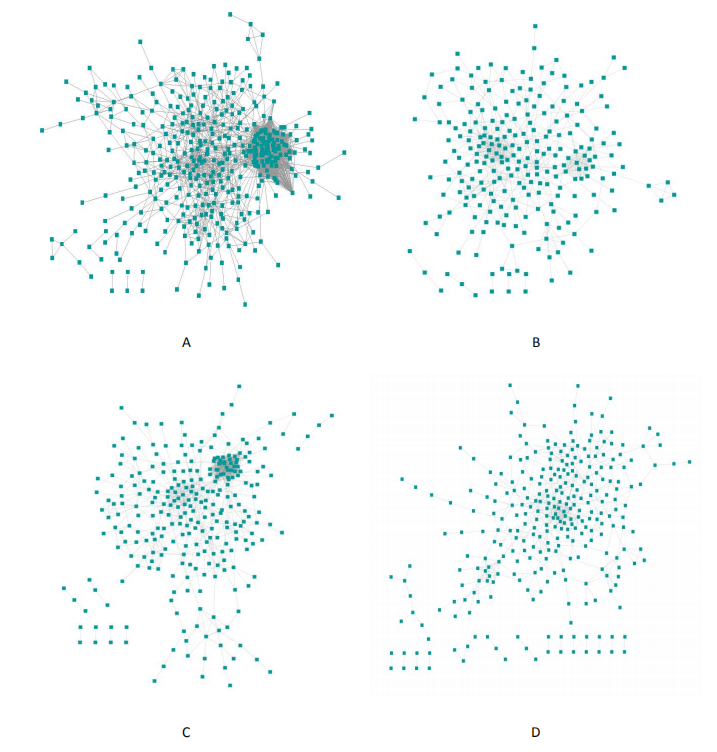
\includegraphics[width=0.98\linewidth,height=0.6\textheight]{FIG/PPI}
	\end{center}
	\caption{ PPI networks of four stages of CRC: vertexs represent the DEGs; edges represent the interactions among genes.\textbf{(A)} is PPI network of DEG-stage1, \textbf{(B)} is PPI network of DEG-stage2, \textbf{(C)} is PPI network of DEG-stage3, \textbf{(D)} is PPI network of DEG-stage4. }\label{PPI}
\end{figure}


\begin{figure}[h]
	\begin{center}
		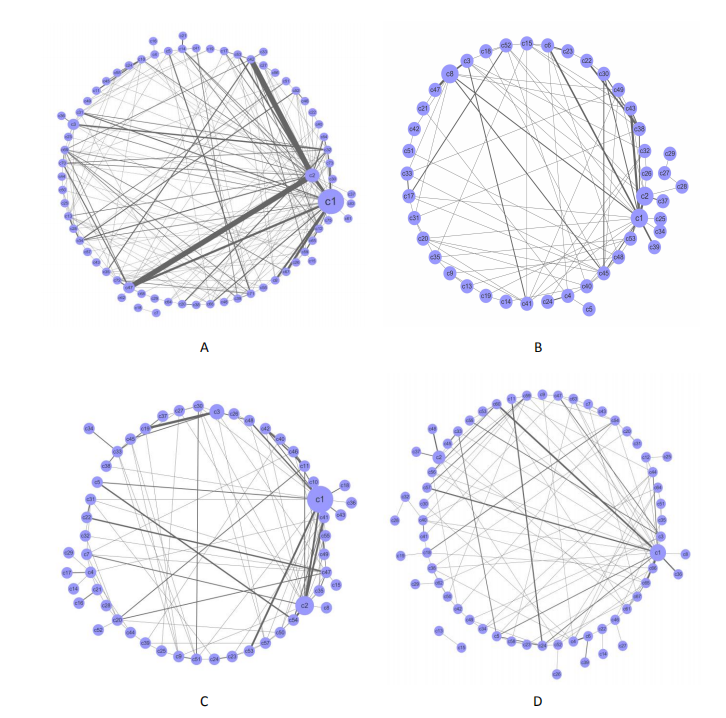
\includegraphics[width=0.98\linewidth,height=0.7\textheight]{FIG/module-network}
	\end{center}
	\caption{ Function module networks of four stages of CRC: vertexs represent the function modules; edges represent the relationship among modules.  \textbf{(A)} is function module network of DEG-stage1, \textbf{(B)} function module network of DEG-stage2, \textbf{(C)} function module network of DEG-stage3, \textbf{(D)} function module network of DEG-stage4.}\label{module-network}
\end{figure}

\begin{figure}[ht]
	\begin{center}
		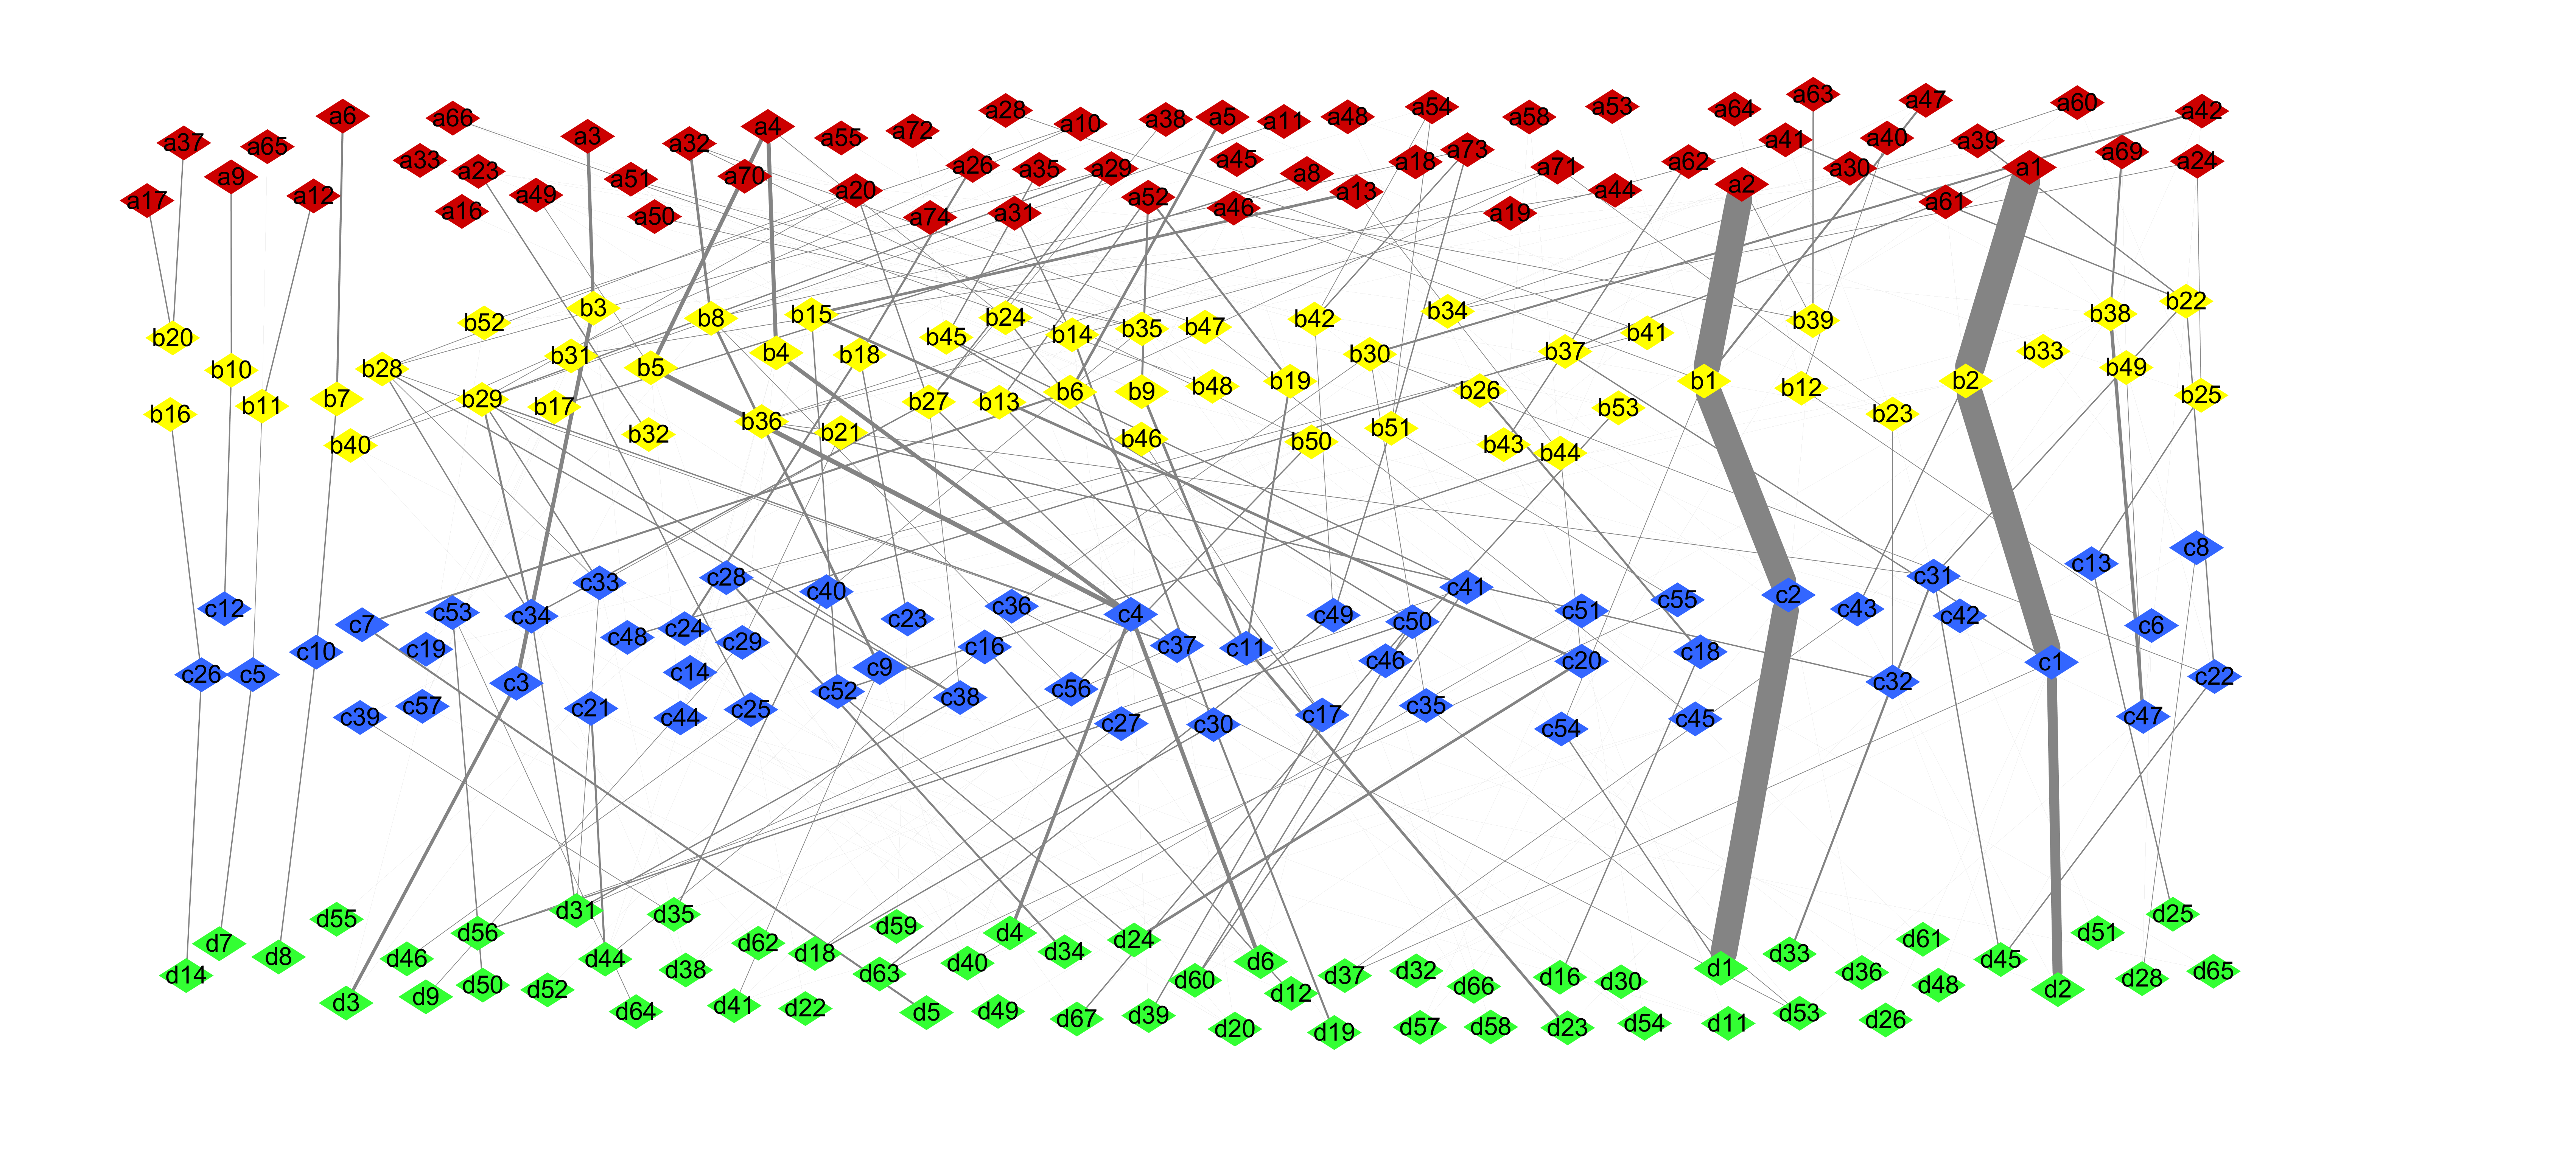
\includegraphics[width=0.98\linewidth,height=0.3\textheight]{FIG/evalution}
	\end{center}
	\caption{ Functional evolution networkbetween adjacent stages of CRC: vertexs represent the function modules; edges represent the relationship among modules. Red, yellow, blue, and green circles represent functional modules belonging to DEG-stage1, DEG-stage2, DEG-stage3, and DEG-stage4, respectively.}\label{evalution}
\end{figure}
\begin{figure}
	\centering
	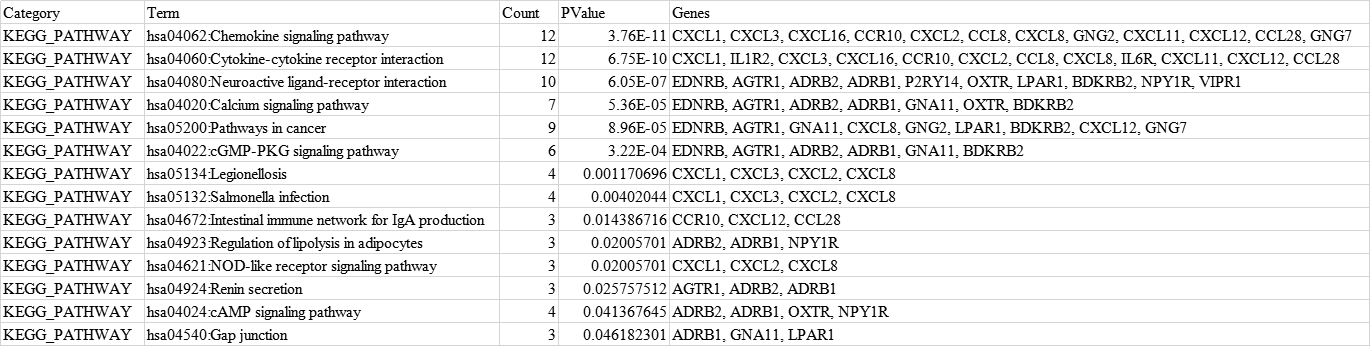
\includegraphics[width=0.98\linewidth]{FIG/screenshot001}
	\caption{KEGG pathways of a2-b1-c2-d1(Mod1)}
	\label{fig:screenshot001}
\end{figure}


\begin{figure}
	\centering
	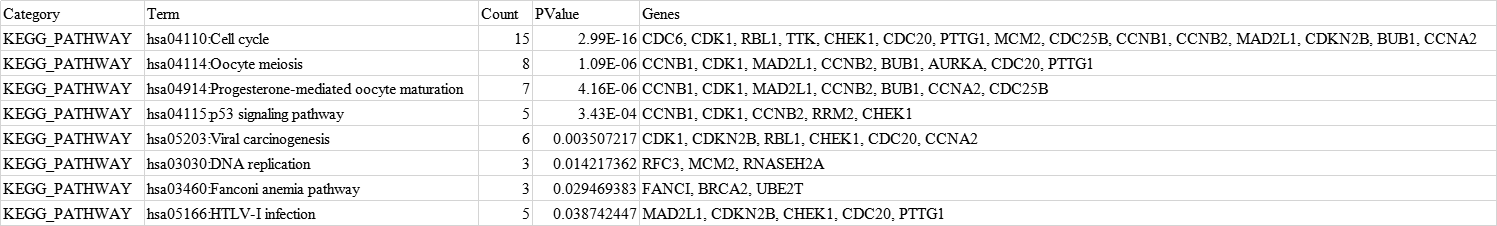
\includegraphics[width=0.98\linewidth]{FIG/screenshot002}
	\caption{KEGG pathways of a1-b2-c1-d2(Mod2)}
	\label{fig:screenshot002}
\end{figure}


\begin{figure}
	\centering
	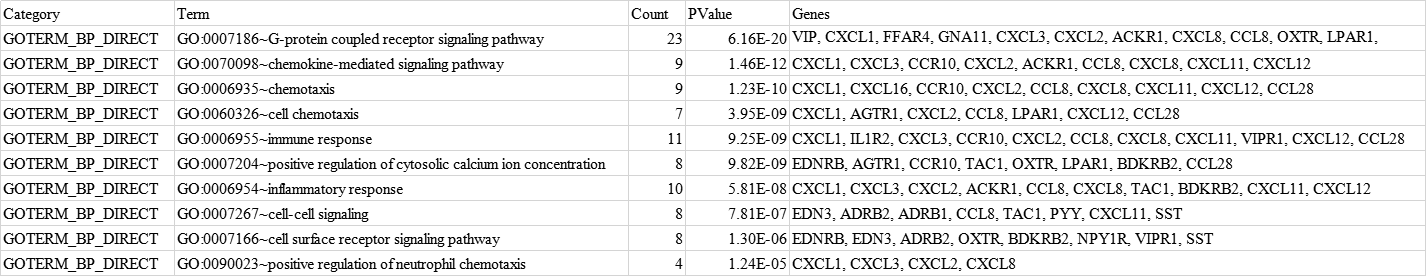
\includegraphics[width=0.98\linewidth]{FIG/screenshot003}
	\caption{Top 10 of GO(BP) term of a2-b1-c2-d1(Mod1)}
	\label{fig:screenshot003}
\end{figure}

\begin{figure}
	\centering
	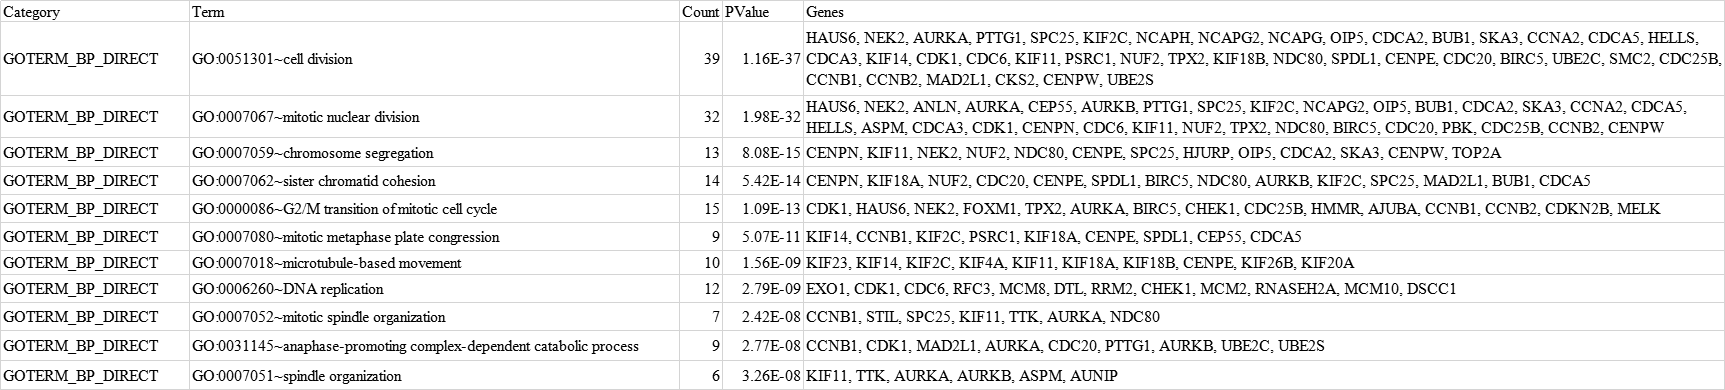
\includegraphics[width=0.98\linewidth]{FIG/screenshot004}
	\caption{Top 10 of GO(BP) term of a1-b2-c1-d2(Mod2)}
	\label{fig:screenshot004}
\end{figure}

%%% Please be aware that for original research articles we only permit a combined number of 15 figures and tables, one figure with multiple subfigures will count as only one figure.
%%% Use this if adding the figures directly in the mansucript, if so, please remember to also upload the files when submitting your article
%%% There is no need for adding the file termination, as long as you indicate where the file is saved. In the examples below the files (logo1.eps and logos.eps) are in the Frontiers LaTeX folder
%%% If using *.tif files convert them to .jpg or .png
%%%  NB logo1.eps is required in the path in order to correctly compile front page header %%%


%%% If you are submitting a figure with subfigures please combine these into one image file with part labels integrated.
%%% If you don't add the figures in the LaTeX files, please upload them when submitting the article.
%%% Frontiers will add the figures at the end of the provisional pdf automatically
%%% The use of LaTeX coding to draw Diagrams/Figures/Structures should be avoided. They should be external callouts including graphics.

\end{document}
